\section{Scope sules}

Yes it is possible to describe it this way. I've modified the program slightly to display the result
of 
\begin{figure}[H]
    \centering
    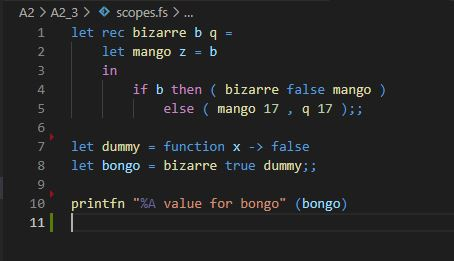
\includegraphics[width=0.75\textwidth]{Figures/Scope_rules.JPG}
    \caption{Modified F\# code from assignment text}
\end{figure}

The result I get in my terminal when running and printing the value of "bongo"
is bongo is = (false, true).

in the body of bongo we have the recursive function bizarre, which get
instansiated with the parameters "true" and "false" since the function dummy
will always set the other parameter to false.

going through the function "bizarre" we can see that the value of b is passed down
until we enter the if statement, where bizarre will be called recursivly and the values
for b and q will be updated with the new value for "b" and the old value for mango which is
"true".